\documentclass[paper=a4, fontsize=10pt]{scrartcl}
\usepackage[bottom=1in, left=1in, right=1in, top=1in]{geometry}
\usepackage{layouts}

\usepackage[usenames,dvipsnames,x11names]{xcolor}

\usepackage[T1]{fontenc}
\usepackage{fourier}
\usepackage[english]{babel}
\usepackage{amsmath,amsfonts,amsthm}

\usepackage{sectsty}
\allsectionsfont{\centering \normalfont\scshape}

\usepackage{tikz}
\usepackage{pgfplots}
\usetikzlibrary{plotmarks}

\usepackage{booktabs}
\usepackage{longtable}
\usepackage{tabularx}
\usepackage{ragged2e}
\newcolumntype{Y}{>{\RaggedRight\arraybackslash}X}
\usepackage{paralist}

\usepackage{acronym}
\usepackage[inline]{enumitem}
\usepackage{fancyhdr}
\usepackage{graphicx}
\usepackage{lastpage}
\usepackage{listings}
\usepackage{multirow}

\pagestyle{fancyplain}
\fancyhead{}
\fancyfoot[L]{}
\fancyfoot[C]{\thepage~of~4}
\renewcommand{\headrulewidth}{0pt}
\renewcommand{\footrulewidth}{0pt}
\setlength{\headheight}{13.6pt}

\newcommand{\horrule}[1]{\rule{\linewidth}{#1}}

\usepackage{algorithm, algpseudocode}
\usepackage{caption}
\usepackage{float}
\usepackage{tabu}

\usepackage{hyperref}
\hypersetup{hidelinks}

\pgfplotsset{compat=1.5}
\usepackage{pgfplots, pgfplotstable}
\usepgfplotslibrary{colorbrewer}

\newacro{MTSP}{Multi-Objective Traveling Salesman Problem}
\newacro{MOEA}{Multi-Objective Evolutionary Algorithm}
\newacro{OX}{Order Crossover}
\newacro{TSP}{Traveling Salesman Problem}

\title{
\normalfont \normalsize
\textsc{Norwegian University of Science and Technology\\IT3708 -- Subsymbolic Methods in AI}
\horrule{0.5pt} \\[0.4cm]
\huge Project 5:\\ Solving \ac{MTSP} using \ac{MOEA}\\
\horrule{2pt} \\[0.5cm]
}

\author{Per Magnus Veierland\\permve@stud.ntnu.no}

\date{\normalsize\today}

\begin{document}

%\fancyfoot[C]{}
\maketitle

\section*{Genotype}

The genotype of a single individual is represented by a vector of integers describing one cyclic \ac{TSP} tour. The vector of integers holds a sequence of $N$ integers, $s_1, s_2, \dots, s_N$, where $N$ is the number of cities in the \ac{TSP}. The sequence is a permutation of the set $\{1, 2, \ldots, N\}$ and describes the order in which to visit each of the cities once. As an example with 5 cities: a sequence $4, 2, 5, 1, 3$ describes a tour starting at city~4, moving to city~2, moving to city~5, moving to city~1, moving to city~3, and finally moving back to starting city~4.

Excluding one city index from the genotype is an option, as one can choose to always visit the city~1 first, and city~1 must always be some place in the sequence. This should reduce the search space without adverse effects. Conclusive results on this design choice were not explored further, and a 48-city genotype ($N=48$) was instead used.

\section*{Crossover}

\setlength\parindent{17pt}

\ac{OX} (Algorithm~\ref{alg:ox}) was introduced by Lawrence Davis in 1985 \cite{davis1985applying}. It is a two-parent ($p_1$ and $p_2$), two-children ($c_1$ and $c_2$) crossover operator intended to preserve the relative ordering of parent genes in offspring. Parents and offspring all share the same genome length, in this context denoted as $N$. Two crossover cut points are selected by first generating two uniformly random integers, \textit{first} and \textit{second} in the range $[0,l]$. The left cutting point is \textsc{min}$(\textit{first}, \textit{second})$, and the right cutting point is \textsc{max}$(\textit{first}, \textit{second})$. Between the cut points, $c_1$ is given the gene values of $p_1$, and $c_2$ is given the gene values of $p_2$.

For the remaining genes, the first child is assigned gene values in order from the second parent, starting from the first gene after the cutting point. Only gene values which are new to the child is assigned; gene values which the child already has are skipped. The same procedure is used to assign gene values from the first parent to the second child. As only gene values which are not already in the child genotype are assigned, and all gene positions in the children are filled, it is clear that children only end up with unique gene values.

Crossover is controlled by a crossover rate, which is a probability between $[0, 1]$ determining whether to apply the crossover operator to produce two children genotypes from two selected parent's genotypes, or to use the parent genotypes unmodified by crossover.

An infeasible child sequence in the context of the \ac{TSP} genotype would be one in which a gene value (i.e. city index) is repeated. As \ac{OX} only produces children where all gene values are unique, provided that the parent gene values are all unique, it is clear that infeasible children cannot be produced.

\begin{algorithm}
\small
\begin{algorithmic}[1]
\Function{Order-Crossover}{$p_1, p_2, \textit{N}$}
    \State let $c_1 \gets$ list of length $N$ with \textit{nil} values; let $c_2 \gets$ list of length $N$ with \textit{nil} values
    \State let $\textit{first} \gets \textsc{RandomInteger}(1, N)$; let $\textit{second} \gets \textsc{RandomInteger}(1, N)$
    \State let $\textit{left} \gets \textsc{min}(\textit{first}, \textit{second})$; let $\textit{right} \gets \textsc{max}(\textit{first}, \textit{second})$
    \For{$m \gets \textit{left}, \textit{right}$}
        \State $c_1[m] \gets p_1[m]$; $c_2[m] \gets p_2[m]$
    \EndFor
    \State $m \gets (\textit{right} + 1) \bmod N$
    \State let $i_1 \gets m$; $i_2 \gets m$
    \While{$m \neq \textit{left}$}
        \While{$p_2[i_2] \in c_1$}
            \State $i_2 \gets (i_2 + 1) \bmod N$
        \EndWhile
        \While{$p_1[i_1] \in c_2$}
            \State $i_1 \gets (i_1 + 1) \bmod N$
        \EndWhile
        \State $c_1[m] \gets p_2[i_2]$; $c_2[m] \gets p_1[i_1]$
    \EndWhile
    \State \textbf{return} $c_1, c_2$
\EndFunction
\end{algorithmic}
\caption{\textsc{Order-Crossover} genetic operator algorithm}
\label{alg:ox}
\end{algorithm}

\section*{Mutation}

The mutation operator is used to maintain genetic diversity in the population. For this problem, a swapping mutation operator was chosen (see Algorithm~\ref{alg:swap}). For a given genotype sequence, $s_1, s_2, \dots, s_N$, two random integer indexes $a$ and $b$ are randomly drawn from a uniform distribution $[1, N]$. The genotype sequence is mutated by swapping the values of genes $s_a$ and $s_b$.

Mutation is controlled by a mutation rate, which is a probability between $[0, 1]$ determining whether to mutate an individual's genotype.

An infeasible child sequence in the context of the \ac{TSP} genotype would be one in which a gene value (i.e. city index) is repeated. As the \textsc{Swap-Mutation} algorithm only swaps two values in a genotype sequence, it will never remove or introduce new values. Therefore, if all values in a sequence is unique before mutating the sequence, it will remain unique after mutating the sequence.

\begin{algorithm}
\small
\begin{algorithmic}[1]
\Function{Swap-Mutation}{$s, N$}
    \State let $a \gets \textsc{RandomInteger}(1, N)$
    \State let $b \gets \textsc{RandomInteger}(1, N)$
    \State let $\textit{t} \gets s[a]$
    \State $s[a] \gets s[b]$
    \State $s[b] \gets \textit{t}$
\EndFunction
\end{algorithmic}
\caption{\textsc{Swap-Mutation} genetic operator algorithm}
\label{alg:swap}
\end{algorithm}

\section*{Selection strategy}

The \ac{MOEA} implementation uses a tournament selection strategy for parent selection. To select a single parent, a random sample of $k$ individuals are drawn from the population $P_t$. With a probability of $\epsilon$, a random individual is selected from the group of $k$ individuals, and with a probability of $1~-~\epsilon$; the lowest ranked individual in the group of $k$ individuals is selected according to the \textit{crowded-comparison operator} $\prec_n$ which is described in NSGA-II \cite{deb2002fast}. This procedure is performed twice to select two parents for each mating which results in two offspring. An $\epsilon$ value of 0.1 was always used.

\section*{Parameter selection}

To evaluate patterns in the effects of parameter selection a parameter search was conducted. For each combination of
\begin{enumerate*}[label=\alph*)]
\item population sizes (50, 100, 500, 1000),
\item group size ratios (0.05, 0.1, 0.2),
\item crossover rates (0, 0.2, 0.4, 0.6, 0.8, 1.0), and
\item mutation rates (0.001, 0.005, 0.01, 0.05, 0.1, 0.5);
\end{enumerate*}
five evolutionary runs were evaluated, for a total of 2160~runs (see Appendix). For each data point the results from five runs are averaged. By combining all the generated solutions, a ``faux Pareto front'' was established and used to calculate estimated convergence and diversity metrics for every non-dominated front. Through interpreting the resulting data it can be concluded that:
\begin{enumerate*}[label=\arabic*)]
\item lower crossover rates and high (but not too high!) mutation rates result in greater diversity,
\item some crossover is necessary for convergence,
\item high crossover rates and low mutation rates result in better extreme solutions, and
\item greater population sizes result in better extreme solutions for the same number of generations.
\end{enumerate*}

To estimate the extremes in the true Pareto front, a 1-tree lower bound \cite{tsplowerbounds} was calculated as 28510 for distance and 134 for cost. As the ``1-tree lower bound'' is usually 10\% below the optimal solution, the optimal distance solution is estimated to be $\approx 31678$, and the optimal cost solution is estimated to be $\approx 149$.

%./create_population_plots.py generated/population-1000-generations-200-group-0.2-crossover-1.0-mutation-0.05-run-2 generated/population-500-generations-200-group-0.05-crossover-1.0-mutation-0.005-run-4 generated/population-100-generations-200-group-0.2-crossover-0.8-mutation-0.005-run-4
%(1000, 200, 0.2, 1.0, 0.05) best_distance=(34869.0, 1693.0) worst_distance=(135113.0, 324.0) best_cost=(135113.0, 324.0) worst_cost=(34869.0, 1693.0) N=1000 ND=1000
%(500, 200, 0.05, 1.0, 0.005) best_distance=(36365.0, 1479.0) worst_distance=(128950.0, 366.0) best_cost=(128950.0, 366.0) worst_cost=(36365.0, 1479.0) N=500 ND=500
%(100, 200, 0.2, 0.8, 0.005) best_distance=(41525.0, 1165.0) worst_distance=(95445.0, 477.0) best_cost=(95445.0, 477.0) worst_cost=(41525.0, 1165.0) N=100 ND=100

\begin{table}
\captionsetup{justification=centering,margin=2cm}
\centering
{\tiny
\begin{tabu} to\linewidth{*{11}{X[c,m]}}
\toprule
Parameter set & Population & Generations & Crossover\newline{}rate & Mutation\newline{}rate & Tournament\newline{}group size & Best distance & Worst distance & Best cost & Worst cost & Non-dominated\newline{}front size \\
\midrule
A &  100 & 200 & 0.8 & 0.005 &  20 & 41525 &  95445 & 477 & 1165 &  100 \\
B &  500 & 200 & 1.0 & 0.005 &  25 & 36365 & 128950 & 366 & 1479 &  500 \\
C & 1000 & 200 & 1.0 & 0.05  & 200 & 34869 & 135113 & 324 & 1693 & 1000 \\
\bottomrule
\end{tabu}
}
\caption{Summary of the top three parameter combinations.}
\label{table:top}
\end{table}

\section*{Comments}

To eliminate a bias introduced by the \texttt{crowding-distance-assignment} function, it was found necessary to shuffle the last front added to the next population. Otherwise, if only part of the last front is added to the next population, having the front sorted by one of the objective functions creates a significant bias towards the lower end of the last objective function sorted for. This in turn can lead to a clustering of solutions on one of the ends of the population front.

As the true Pareto front is unknown to the implementation for the problem given, $f^\text{max}_m$ and $f^\text{min}_m$ are estimated for each objective function $m$ by tracking the maximum and minimum values encountered throughout an evolutionary run for each objective.

\begin{figure}[H]
\centering
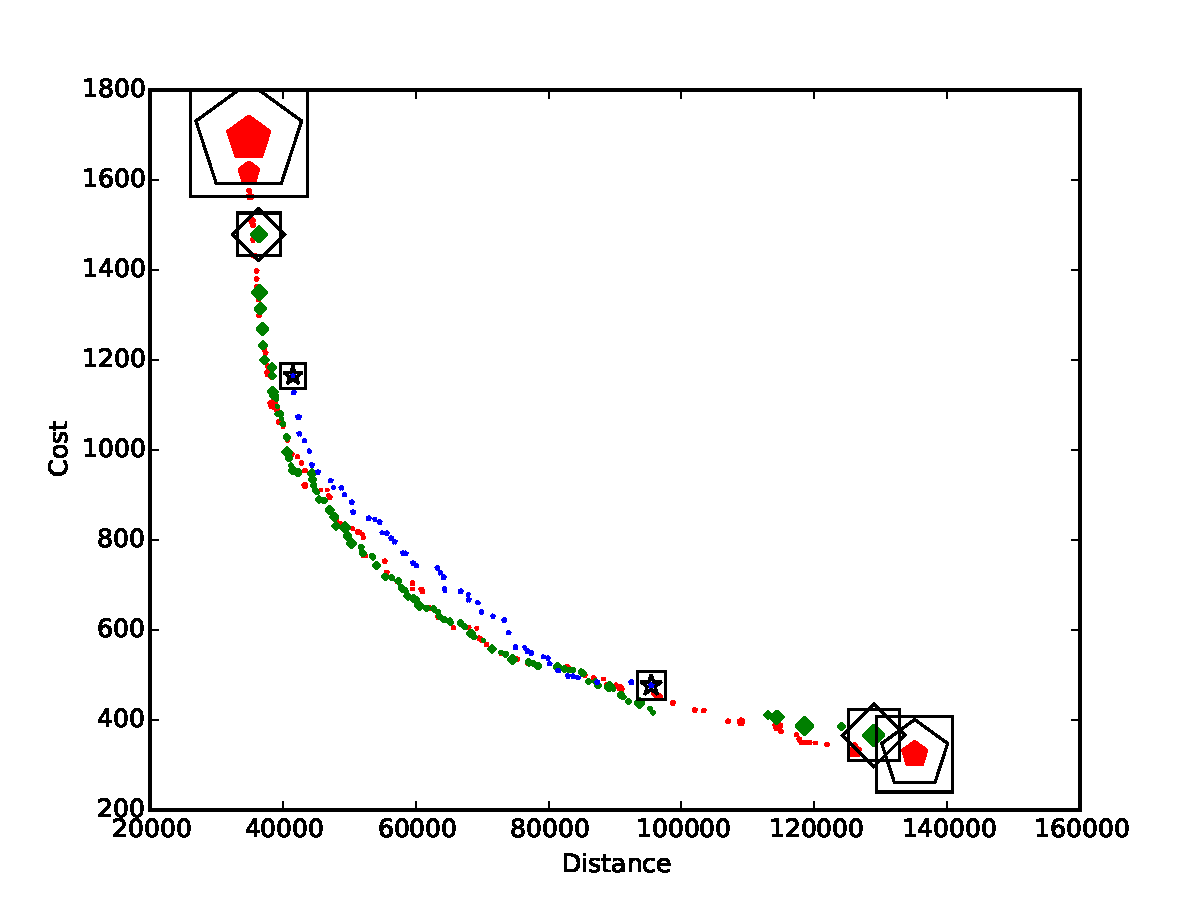
\includegraphics[width=0.7\textwidth]{figures/all-nd-fronts}
\caption{Non-dominated fronts for parameter~set~A~(blue stars), parameter~set~B~(green diamonds), parameter~set~C~(red pentagons). Shape sizes indicates clustered solutions. Shape outlines indicates best solution for an objective while square outlines indicates worst solution for an objective.}
\end{figure}

\begin{figure}[H]
\centering
\begin{tabular}{cc}
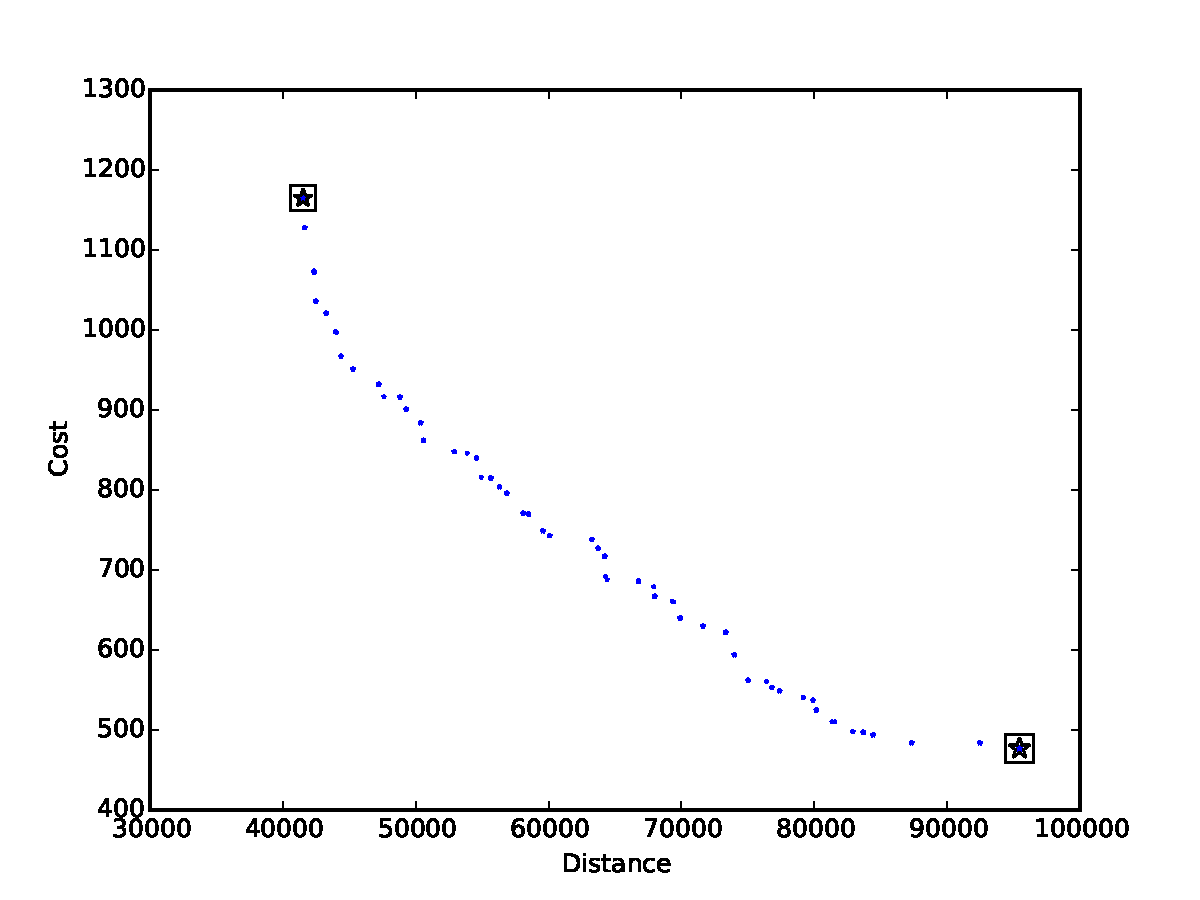
\includegraphics[width=0.4\textwidth]{figures/population-100-generations-200-group-0-2-crossover-0-8-mutation-0-005-run-4-front} &
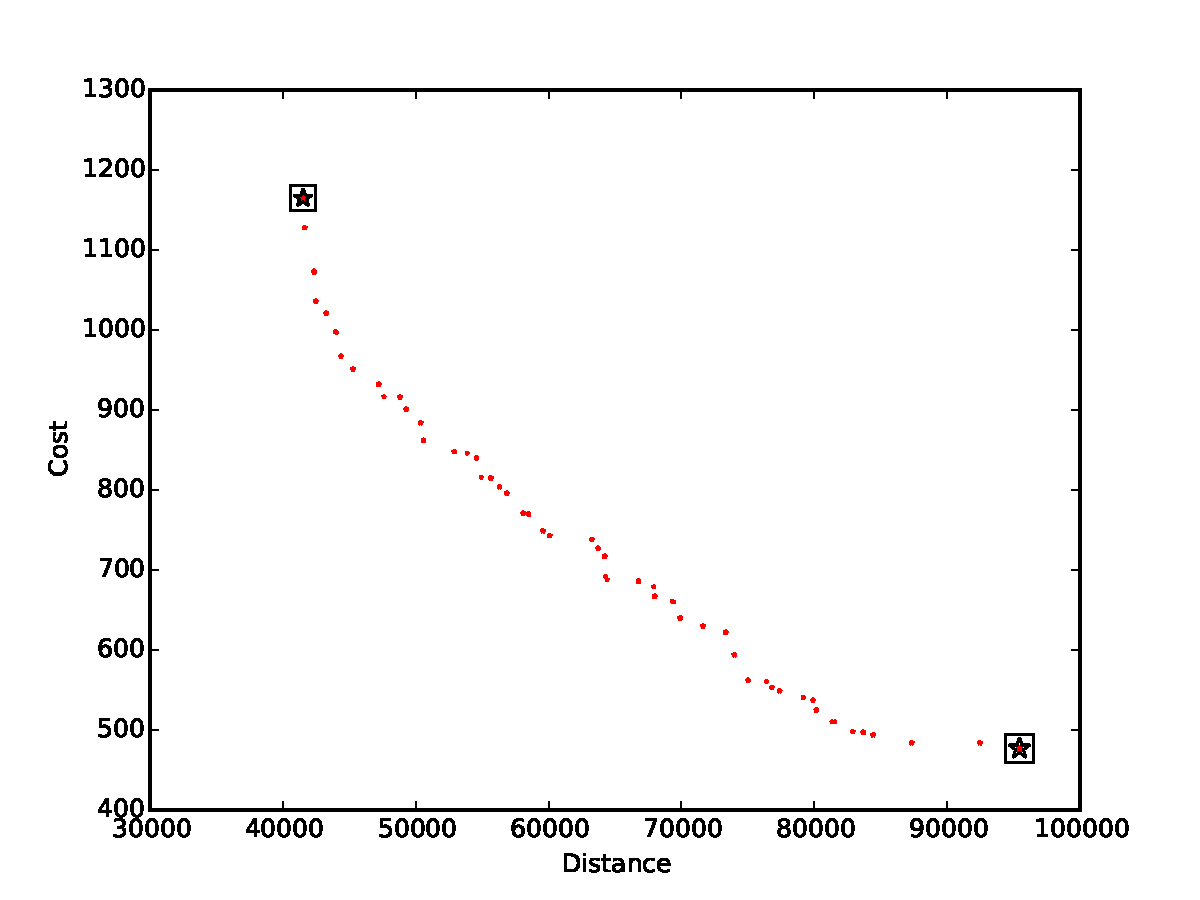
\includegraphics[width=0.4\textwidth]{figures/population-100-generations-200-group-0-2-crossover-0-8-mutation-0-005-run-4-population} \\
\end{tabular}
\caption{Non-dominated front (\textit{left}) and full population (\textit{right}) for parameter set A.}
\end{figure}

\begin{figure}[H]
\centering
\begin{tabular}{cc}
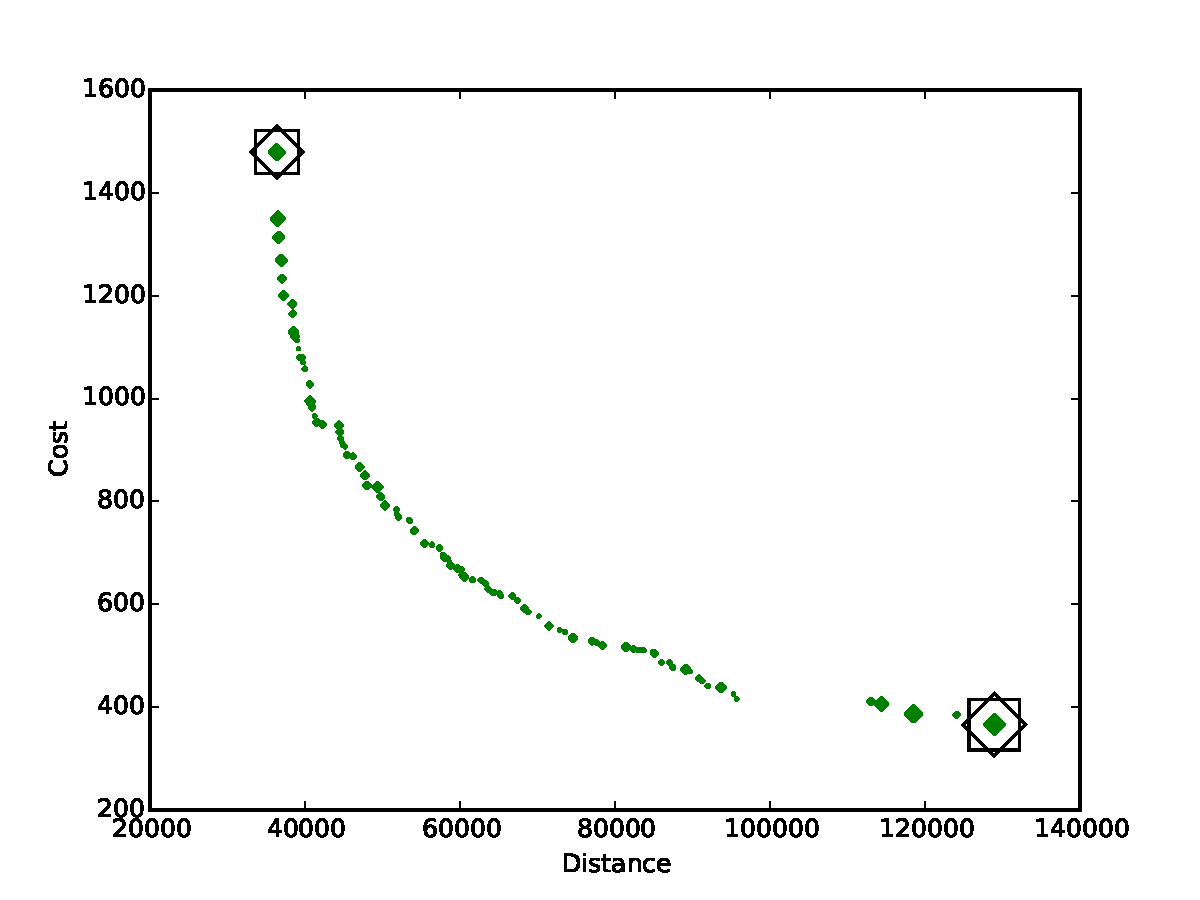
\includegraphics[width=0.4\textwidth]{figures/population-500-generations-200-group-0-05-crossover-1-0-mutation-0-005-run-4-front} &
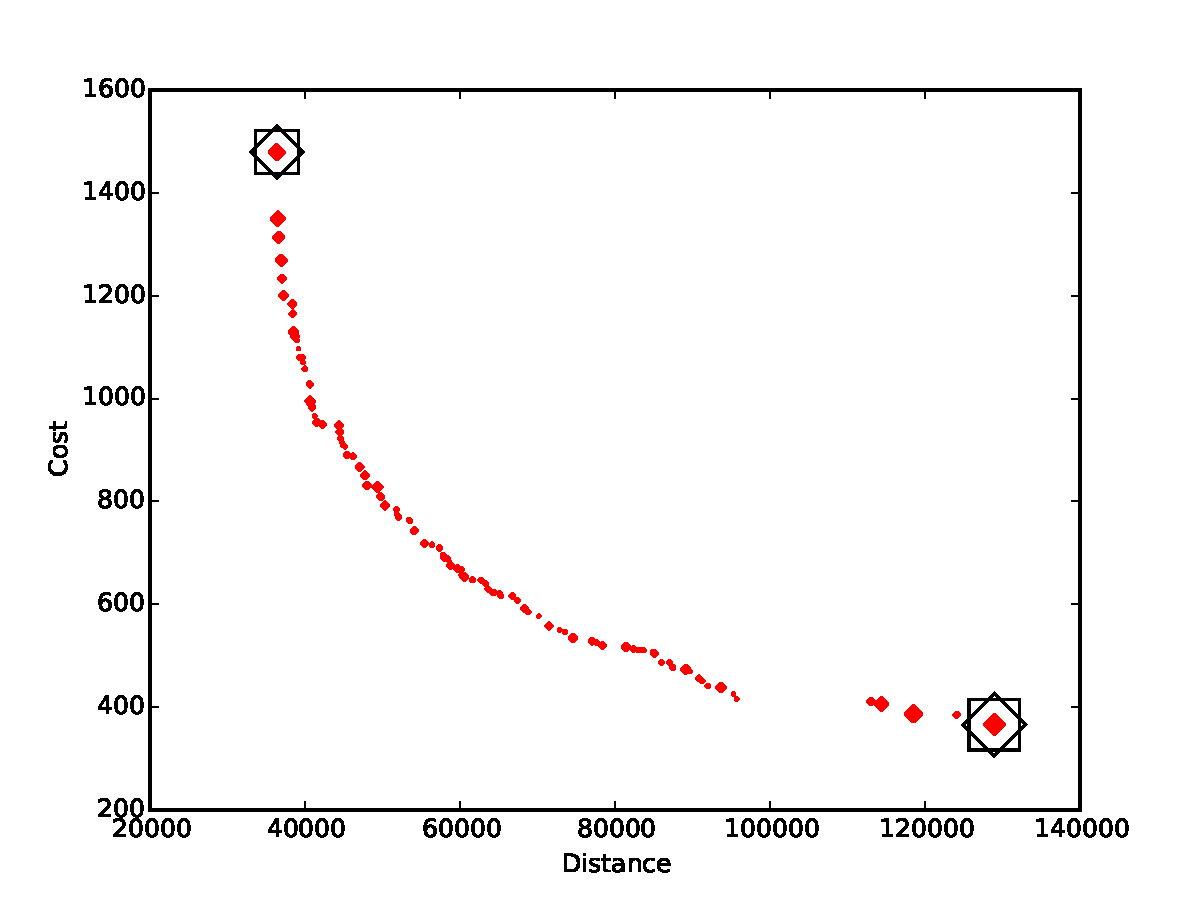
\includegraphics[width=0.4\textwidth]{figures/population-500-generations-200-group-0-05-crossover-1-0-mutation-0-005-run-4-population} \\
\end{tabular}
\caption{Non-dominated front (\textit{left}) and full population (\textit{right}) for parameter set B.}
\end{figure}

\begin{figure}[H]
\centering
\begin{tabular}{cc}
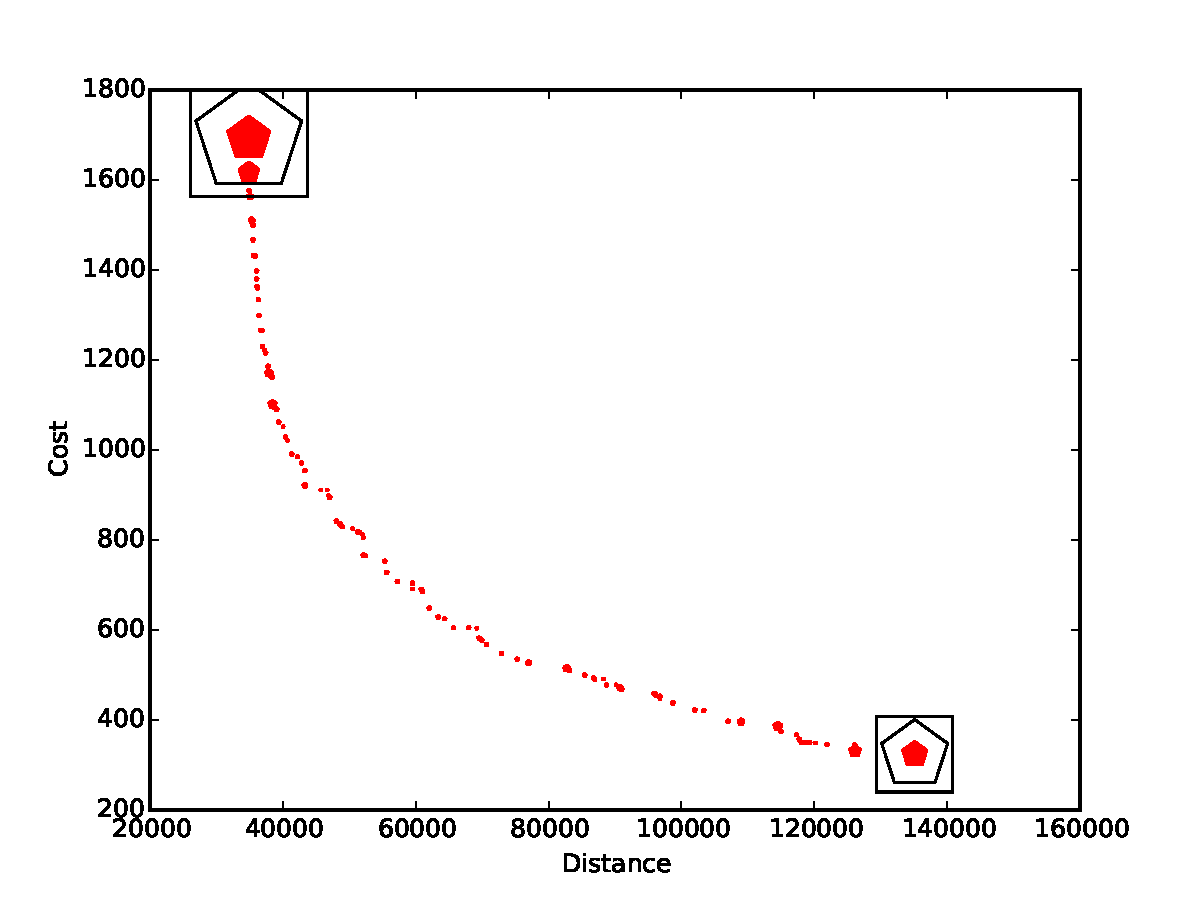
\includegraphics[width=0.4\textwidth]{figures/population-1000-generations-200-group-0-2-crossover-1-0-mutation-0-05-run-2-front} &
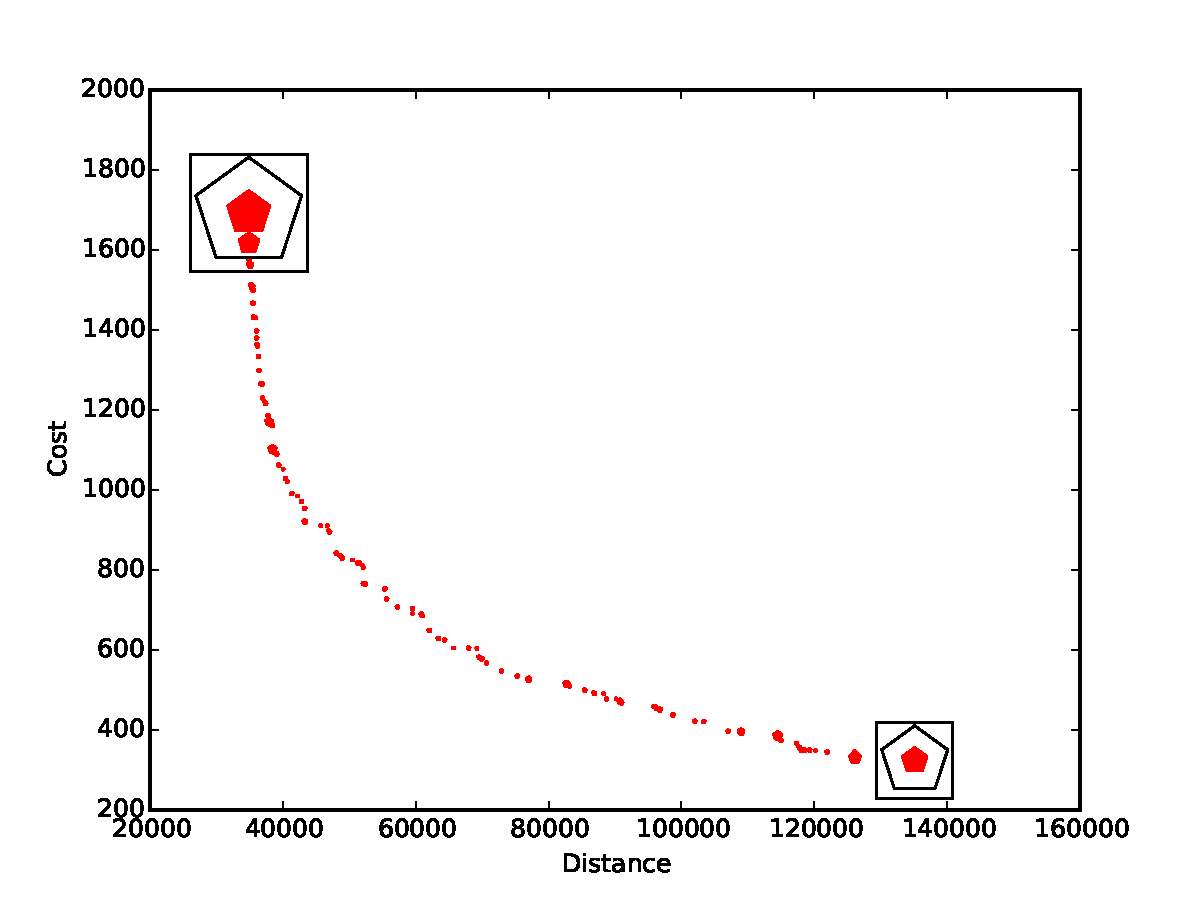
\includegraphics[width=0.4\textwidth]{figures/population-1000-generations-200-group-0-2-crossover-1-0-mutation-0-05-run-2-population} \\
\end{tabular}
\caption{Non-dominated front (\textit{left}) and full population (\textit{right}) for parameter set C.}
\end{figure}

\bibliographystyle{unsrt}
\bibliography{references}

\newcommand{\displayplot}[4]{
    \begin{tikzpicture}[scale=0.5]
    \begin{axis}[view={0}{90},
        xlabel=Crossover Rate,
        ylabel=Mutation Rate,
        ymode=log,
        title=#4,
        log ticks with fixed point,
        y tick label style={/pgf/number format/1000 sep=\,},
        colormap name=#3,
        colorbar,
        colorbar horizontal,
        colorbar style={
            at={(0, -0.4)},
            anchor=south west,
            title=Value,
            ticklabel style={
                scaled ticks=false,
                /pgf/number format/fixed
            }
        }]
    \addplot3[surf] table[x index=0,y index=1,z index=#2] {#1};
    \end{axis}
    \end{tikzpicture}
}

\pgfplotsset{
colormap={Blues-9-Inv}{
  color=(Blues-9-9);
  color=(Blues-9-8);
  color=(Blues-9-7);
  color=(Blues-9-6);
  color=(Blues-9-5);
  color=(Blues-9-4);
  color=(Blues-9-3);
  color=(Blues-9-2);
  color=(Blues-9-1);
},
colormap={Purples-9-Inv}{
  color=(Purples-9-9);
  color=(Purples-9-8);
  color=(Purples-9-7);
  color=(Purples-9-6);
  color=(Purples-9-5);
  color=(Purples-9-4);
  color=(Purples-9-3);
  color=(Purples-9-2);
  color=(Purples-9-1);
}}

\newcommand{\displayplots}[4]{
    \displayplot{plots/population-#2-generations-#3-group-#4}{2}{PiYG-11}{Diversity} &
    \displayplot{plots/population-#2-generations-#3-group-#4}{3}{RdBu-11}{Convergence} &
    \displayplot{plots/population-#2-generations-#3-group-#4}{4}{Blues-9-Inv}{Distance (min)} &
    \displayplot{plots/population-#2-generations-#3-group-#4}{5}{Purples-9-Inv}{Cost (min)} \\[0.25cm]
    \multicolumn{4}{c}{\textbf{Figure #1:} Population: #2 -- Generations: #3 -- Group Ratio: #4} \\[2cm]
}

\newgeometry{left=1cm,right=1cm,top=3cm,bottom=1cm}

\section*{Appendix: Parameter search}

\begin{table}[H]
\centering
\begin{tabular}{cccc}
\displayplots{1}{50}{200}{0.05}
\displayplots{2}{50}{200}{0.1}
\displayplots{3}{50}{200}{0.2}
\end{tabular}
\end{table}

\begin{table}[H]
\centering
\begin{tabular}{cccc}
\displayplots{4}{100}{200}{0.05}
\displayplots{5}{100}{200}{0.1}
\displayplots{6}{100}{200}{0.2}
\end{tabular}
\end{table}

\begin{table}[H]
\centering
\begin{tabular}{cccc}
\displayplots{7}{500}{200}{0.05}
\displayplots{8}{500}{200}{0.1}
\displayplots{9}{500}{200}{0.2}
\end{tabular}
\end{table}

\begin{table}[H]
\centering
\begin{tabular}{cccc}
\displayplots{10}{1000}{200}{0.05}
\displayplots{11}{1000}{200}{0.1}
\displayplots{12}{1000}{200}{0.2}
\end{tabular}
\end{table}

\end{document}

